\section{项目的主要内容和技术路线}

\subsection{主要研究内容}
本项目主要研究样条曲线拟合,
主要包括离散最小二乘样条逼近
(discrete least squares splines approximation)
与平滑样条拟合(smoothing splines fitting)
的相关理论和编程实现。
\subsubsection{离散最小二乘样条逼近}
离散最小二乘样条逼近旨在解决如下问题:
已知$\mathbf{x}=\{x_{i}\}_{i=1}^{N},\ \mathbf{y}=\{y_{i}\}_{i=1}^{N},
\ \mathbf{w}=\{w_{i}\}_{i=1}^{N}$,其中
$x_{i}$关于$i$严格递增,$w_{i}>0$。
同时,已知递增节点组$\{t_{i}\}_{i=1}^{n+k}$。
我们需要找到一个$k$阶 B 样条函数$f$,使得
\begin{equation}
  \label{eq:DiscreteLeastSquaresSplinesApproximation}
  \sum_{i=1}^{N}w_{i}(y_{i}-f(x_{i}))^{2}
\end{equation}
取得最小值。与这个问题相对应的是 Matlab 曲线拟合工具箱中的 spap2 函数。

这个$f$存在的前提是,存在$\mathbf{x}$的子列$\{x_{j_{i}}\}_{i=1}^{n}$,
其满足 Schoenberg-Whitney 条件:
\begin{equation}
  \label{eq:SWcondition}
  t_{i}<x_{j_{i}}<t_{i+k},\quad i=1,2,\cdots,n.
\end{equation}

其次,$f$所在的空间为$\text{span}\{B_{2},B_{3},\cdots,B_{n+1}\}$,
其中$B_{j+1}$为节点$t_{j},t_{j+1},\cdots,t_{j+k}$所对应的基函数,具体地,
\begin{equation}
  \label{eq:basicBSpline}
  B_{j+1}(x)=
  (t_{j+k}-t_{j})\cdot [t_{j},t_{j+1},\cdots,t_{j+k}](t-x)_{+}^{k-1},
\end{equation}
$[t_{j},t_{j+1},\cdots,t_{j+k}]g$为
$g$关于$\{t_{j+i}\}_{i=0}^{k}$的$k$阶差商($k$th divided difference),
\begin{equation}
  \label{eq:truncatedPowerFunc}
  t_{+}^{m}=
  \left\lbrace
    \begin{aligned}
      t^{m},\ t&\ge 0,\\
      0,\ t&<0
    \end{aligned}
  \right.
\end{equation}
为截断幂函数(truncated power function)。

\subsubsection{平滑样条拟合}
平滑样条拟合旨在通过对数据点插值得到的曲线
以及通过最小二乘法得到的曲线中作出平衡,以得到一条平滑曲线。
目前较为经典的平滑样条拟合有两种,
一种为 pp 格式的三次平滑样条拟合,
一种为 B 格式的$2m$阶(即$2m-1$次)平滑样条拟合。
  
针对三次平滑样条拟合,其主要问题为:
已知$\mathbf{x}=\{x_{i}\}_{i=1}^{N},\ \mathbf{y}=\{y_{i}\}_{i=1}^{N},
\ \mathbf{w}=\{w_{i}\}_{i=1}^{N}$,$p\in [0,1]$,其中
$x_{i}$关于$i$严格递增,$w_{i}>0$。
同时,已知$\lambda(t)$
是在$[x_{1},x_{N}]$上关于$\mathbf{x}$的分片常值函数,即
\begin{equation}
  \label{eq:lambdatx}
  \lambda(t)\equiv \lambda_{i}\ge 0,\
  t\in [x_{i},x_{i+1}],\quad i=1,2,\cdots,N-1.
\end{equation}
我们需要找到一个自然边界条件(即满足$f''(x_{1})=f''(x_{N})=0$的$f$)
下的三次 pp 样条函数$f$,使得
\begin{equation}
  \label{eq:cubicSmoothingSplinesFitting}
  p\sum_{i=1}^{N}w_{i}(y_{i}-f(x_{i}))^{2}+
  (1-p)\int_{x_{1}}^{x_{N}}\lambda(t)|f''(t)|^{2}\mathrm{d}t
\end{equation}
取得最小值。与这个问题相对应的是 Matlab 曲线拟合工具箱中的 csaps 函数。
当$\lambda\equiv1$时,有较为经典的求解方法
\cite{GuideToSplines}。
对于$\lambda$不恒等于1的情形,通过图~\ref{fig:cubicSplinesSpaceCompare}
中对比 Matlab 中样条曲线的结果,我们发现
$f$并没有落在通常的
\begin{equation}
  \label{eq:cubicSplinesSpace}
  \mathbb{S}_{3}^{2}(\mathbf{x}):=\{g\in C^{2}([x_{1},x_{N}]):
  \ g|_{[x_{i},x_{i+1}]}\in \mathbb{P}_{3},\ i=1,2,\cdots,N-1\}
\end{equation}
空间中,而是落在如下的空间中:
\begin{equation}
  \label{eq:cubicSplinesSpaceLambda}
  \mathbb{S}_{3}^{2}(\mathbf{x};\lambda)
  :=\{g\in D^{2}([x_{1},x_{N}]):
  \ \lambda g''\in C([x_{1},x_{N}]),
  \ g|_{[x_{i},x_{i+1}]}\in\mathbb{P}_{3},
  \ i=1,2,\cdots,N-1\}.
\end{equation}
因此,针对这个问题,我们需要先研究清楚在$\mathbb{S}_{3}^{2}(\mathbf{x};\lambda)$
空间中样条函数的性质,
以及其与$\mathbb{S}_{3}^{2}(\mathbf{x})$经典空间中样条函数性质的不同。
然后再试图仿照经典的求解方法得到此问题的求解方法。

\begin{figure}[h]  
  \centering   
  \begin{minipage}{0.42\textwidth}  
    \centering  
    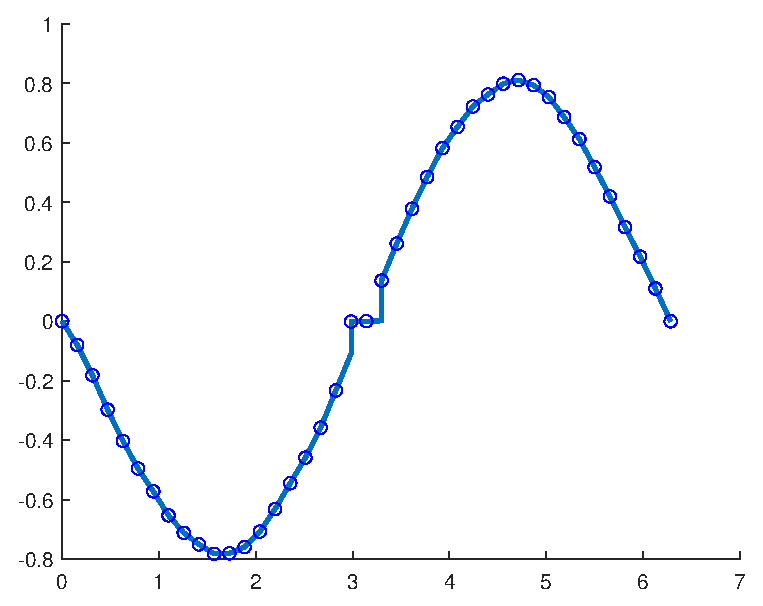
\includegraphics[width=\linewidth]{eps/fDeriv2.eps}  
    \caption*{$f''$的图像,在$\lambda_{i}\neq 1$附近的点上不连续}  
  \end{minipage}  
  \hfill  
  \begin{minipage}{0.42\textwidth}  
    \centering  
    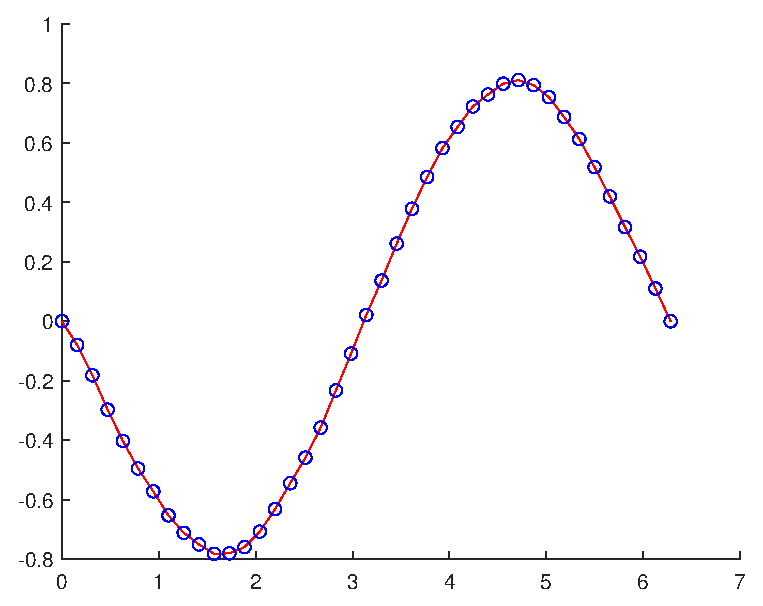
\includegraphics[width=\linewidth]{eps/lamfDeriv2.eps}  
    \caption*{$\lambda f''$的图像,在$[x_{1},x_{N}]$上是连续的}  
  \end{minipage}    
  \caption{ Matlab 中通过 csaps 函数得到的样条$f$,
    其中$\lambda_{i}$在中间两段区间上取值为100,在其余区间上取值为1。}
  \label{fig:cubicSplinesSpaceCompare}  
\end{figure}

针对$2m$阶平滑样条拟合,
其主要问题为:
已知$\mathbf{x}=\{x_{i}\}_{i=1}^{N},\ \mathbf{y}=\{y_{i}\}_{i=1}^{N},
\ \mathbf{w}=\{w_{i}\}_{i=1}^{N}$,其中
$x_{i}$关于$i$严格递增,$w_{i}>0$。
同时,已知$S\ge 0$,$\lambda(t)$满足~(\ref{eq:lambdatx})。
我们需要找到一个自然边界条件
(即满足$D^{j}f(x_{1})=D^{j}f(x_{N})=0,\ j=m,m+1,\cdots,2m-2$的$f$)
下的$2m$阶 B 样条函数$f$,
使得$E(f):=\sum_{i=1}^{N}w_{i}(y_{i}-f(x_{i}))^{2}\le S$且
\begin{equation}
  \label{eq:FDmf}
  F(D^{m}f):=\int_{x_{1}}^{x_{N}}\lambda(t)|D^{m}f(t)|^{2}\mathrm{d}t
\end{equation}
取到最小值。与这个问题相对应的是 Matlab 曲线拟合工具箱中的 spaps 函数。
同时,解决此问题后,
我们还能得到一个平滑参数(smoothing parameter)$\rho$,
它使得$f$被确定为表达式$\rho E(f) + F(D^m f)$的唯一最小化函数,
且使得$E(f)=S$成立。
由于样条函数的分片多项式不需要太高的阶数,结合 Matlab 的函数实现,
在本项目的工作中,我们仅编程实现$m=1,2,3$的情形。

\subsection{技术路线}
本文所使用的代码语言均为 C++。

先构建样条基类以及其两个派生类 pp 样条与 B 样条,
使它们分别有基本的功能。

针对离散最小二乘样条逼近问题,需要得到一个 B 样条,
它是一些 B 样条基函数的线性组合。
此问题可以转化为求解一个超定方程组,其中系数矩阵为
%样条配置矩阵(spline collocation matrix)。该矩阵是
几乎块对角矩阵(almost block-diagonal matrix),
可以对其进行块 QR 分解(block QR factorization)
\cite{Boor1976SOLVEBLOKAP},从而在最小二乘意义下求出方程组的解。

针对三次平滑样条拟合问题,需要得到一个自然边界条件下的三次 pp 样条。
考虑到$\lambda$可能不恒为1的情况,我们需要重新理解
三次样条在数据点上二阶导数值与函数值之间的关系,并应用到现有的求解
方法\cite{GuideToSplines}上进行改进更新。最终得到的线性方程组的系数矩阵
仍是对称正定的五对角矩阵,可以对其使用 $LDL^{T}$ 分解,进一步求出
此线性方程组的解。

针对$2m$阶平滑样条拟合问题,需要得到一个自然边界下的$2m$阶 B 样条。
目前考虑按照 de Boor \cite{Boor2001CALCULATIONOT}的方法进行实现,
然后对一个关于平滑参数$\rho$的方程使用 Newton 法求根,以计算$\rho$的值
\cite{SmoothingBySplineFunctions}。

\subsection{可行性分析}
目前我们已经有比较丰富的代码基础。具体地,我们已经构建了
pp 样条和 B 样条两个派生类,并实现了它们的一些基本功能。
我们已经实现了
B 样条插值函数(对应于Matlab 曲线拟合工具箱中的 spapi 函数),
此问题可以转化为求解一个线性方程组,
其中系数矩阵为几乎块对角的方阵,也可以进行块 QR 分解。
因此,我们可以仿照这个过程,编写离散最小二乘样条逼近问题对应的代码。

对于三次平滑样条拟合,
我们已经有了$\lambda\equiv1$情形的理论以及编程算法。
对其进行改进,可以得到对一般$\lambda$的理论以及编程算法。
当系数矩阵进行 $LDL^{T}$ 分解后,对于所要求解的各种
系数矩阵为三角矩阵的方程,也已经有了相关的代码实现。

对于$2m$阶平滑样条拟合问题,也有相关理论进行支撑
\cite{Boor2001CALCULATIONOT,SmoothingBySplineFunctions}。
接下来只需掌握其理论,并给出相应算法和编程实现即可。

在所有代码编写完毕后,我们将此代码转化为
适应北太天元接口的代码。在进行充分的测试后,将其和北太天元的接口进行对接。
